\documentclass{article}
\usepackage[margin=1in]{geometry}
\usepackage{amsmath,amsthm,amssymb}
\usepackage{bbm,enumerate,mathtools}
\usepackage{tikz,pgfplots}
\usepackage{chessboard}
\usepackage[hidelinks]{hyperref}
\usepackage{multicol} % Problem 35

\newenvironment{question}{\begin{trivlist}\item[\textbf{Question.}]}{\end{trivlist}}
\newenvironment{note}{\begin{trivlist}\item[\textbf{Note.}]}{\end{trivlist}}
\newenvironment{references}{\begin{trivlist}\item[\textbf{References.}]}{\end{trivlist}}
\newenvironment{related}{\begin{trivlist}\item[\textbf{Related.}]\end{trivlist}\begin{enumerate}}{\end{enumerate}}


\begin{document}

\rating{2}{2}
There are two popular, essentially identical, iPhone games in the app store:
\textit{AMAZE!!!} and \textit{Roller Splat!}.
The goal of the puzzle is to reach every (white) square in the board---the catch
is that you can only move in as-long-as-possible rook moves.
\begin{figure}[ht!]
  \centering
  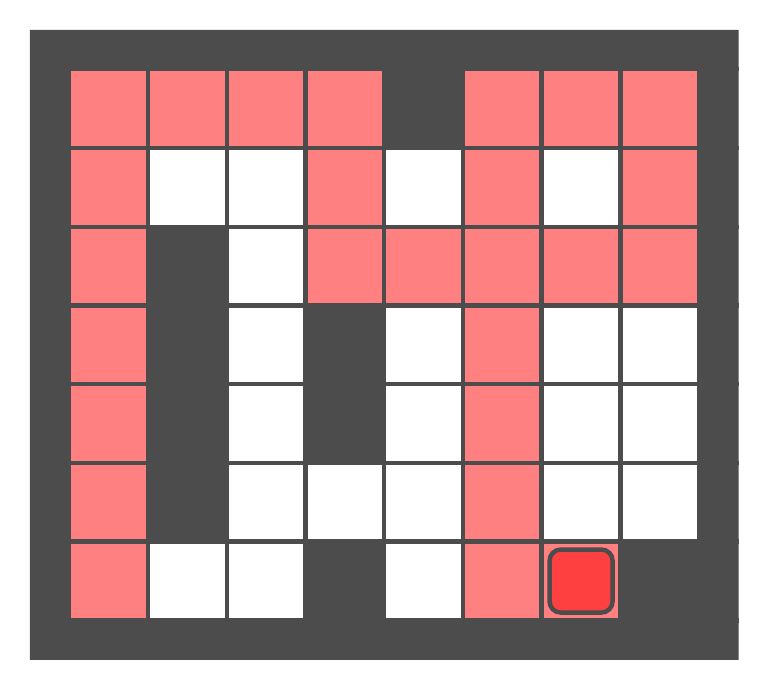
\begin{tikzpicture}
    \draw[line width=27,red!50] (1.5,1)--(1.5,7.5)--(4.5,7.5)--(4.5,5.5)--(8.5,5.5)--(8.5,7.5)--(6.5,7.5)--(6.5,1.5)--(8,1.5);
    \draw[black!70, ultra thick] (0.5,0.5) grid (9.5,8.5);
    \fill[black!70]
      (9.5,1) rectangle (0.5,0.5) rectangle (1,8.5)
      (9,0.5) rectangle (9.5,8.5) rectangle (0.5,8)
      (2,2) rectangle (3,6)
      (4,0.5) rectangle (5,2)
      (4,3) rectangle (5,5)
      (6,8.5) rectangle (5,7)
      (8,0.5) rectangle (9,2)
    ;
    \draw[black!70, ultra thick, rounded corners, fill=red!75] (7.1,1.1) rectangle (7.9,1.9);
  \end{tikzpicture}
  \caption{
    Starting from the lower left corner, the board can be filled using the following $25$ moves: $
      \protect\underbrace{
        \uparrow\rightarrow\downarrow\rightarrow\uparrow\leftarrow\downarrow\rightarrow
      }_\text{illustrated above}
      \uparrow\downarrow\leftarrow\uparrow\leftarrow\rightarrow\downarrow\leftarrow\uparrow\downarrow\leftarrow
    $
  }
\end{figure}

\begin{question}
  How many solvable puzzles exist on an $n \times m$ board?
\end{question}

\begin{related}
  \item What if we only want to count ``primitive'' puzzles---those that cannot
  exist on a smaller board?
  \item What if we count up to symmetries of the rectangle?
  \item Which puzzle requires the greatest number of moves?
  \item What if we do this on a torus? M\"obius strip? More dimensions?
  \item Given some configuration, what is an algorithm to figure out how to solve it?
\end{related}

\end{document}
